\NeedsTeXFormat{LaTeX2e}
\documentclass[a4paper,12pt,
headsepline,           % Linie zw. Kopfzeile und Text
oneside,               % einseitig
pointlessnumbers,      % keine Punkte nach den letzten Ziffern in Überschriften
bibtotoc,              % LV im IV
%DIV=15,               % Satzspiegel auf 15er Raster, schmalere Ränder   
%BCOR15mm               % Bindekorrektur
%,draft
]{scrartcl}

\usepackage{amsmath}
\usepackage{amsfonts}
\usepackage{amssymb}
\usepackage{enumitem}
\usepackage[utf8]{inputenc} % this is needed for umlauts
\usepackage[ngerman]{babel} % this is needed for umlauts
\usepackage[T1]{fontenc} 
\usepackage{commath}
\usepackage{xcolor}
\usepackage{booktabs}
\usepackage{float}
\usepackage{tikz-timing}
\usepackage{tikz}
\usepackage{multirow}
\usepackage[final]{pdfpages}
\usepackage{blindtext}
\usepackage{listings}
\usepackage[scaled]{helvet}
\usepackage{hyperref}
\usepackage{comment}
\usepackage{mathtools}
\DeclarePairedDelimiter{\ceil}{\lceil}{\rceil}

\usetikzlibrary{calc,shapes.multipart,chains,arrows}

\KOMAoptions{DIV=last} % Neuberechnung Satzspiegel nach Laden von Paket helvet

\usepackage{scrpage2}
\pagestyle{useheadings}

\renewcommand{\familydefault}{\sfdefault} 

\setlength{\parindent}{0pt}   % kein linker Einzug der ersten Absatzzeile
\setlength{\parskip}{1.4ex plus 0.35ex minus 0.3ex} % Absatzabstand, leicht variabel

\newcommand{\fullname}{Gruppe 10}
\newcommand{\titel}{Softwaregrundprojekt Meilenstein 6}
\newcommand{\jahr}{2019}
\newcommand{\dozent}{Florian Ege}
\newcommand{\betreuer}{Stefanos Mytilineos}
\newcommand{\fakultaet}{Ingenieurwissenschaften, Informatik und\\Psychologie}
\newcommand{\institut}{Institut für Softwaretechnik und Programmiersprachen}

\pdfinfo{
    /Author (\fullname)
    /Title (\titel)
    /Producer     (pdfeTex 3.14159-1.30.6-2.2)
    /Keywords ()
}

\hypersetup{
    pdftitle=\titel,
    pdfauthor=\fullname,
    pdfsubject={Softwaregrundprojekt-Abgabe},
    pdfproducer={pdfeTex 3.14159-1.30.6-2.2},
    colorlinks=false,
    pdfborder=0 0 0	% keine Box um die Links!
}

% Trennungsregeln
\hyphenation{Sil-ben-trenn-ung}

\makeatletter
\@addtoreset{section}{part}
\makeatother

\begin{document}
    \thispagestyle{empty}
    \begin{addmargin*}[4mm]{-10mm}

        
\includegraphics[height=1.8cm]{images/unilogo_bild}
        \hfill
        
\includegraphics[height=1.8cm]{images/unilogo_wort}\\[1em]

        {\footnotesize
        %{\bfseries Universität Ulm} \textbar ~89069 Ulm \textbar ~Germany
        \hspace*{115mm}\parbox[t]{35mm}{\bfseries Fakultät für\\
        \fakultaet\\
        \mdseries \institut}\\[2cm]

        \parbox{140mm}{\bfseries \LARGE \titel}\\[2.5em]
        {\footnotesize Softwaregrundprojekt an der Universität Ulm}\\[3em]

        {\footnotesize \bfseries Vorgelegt von:}\\
        {\footnotesize \fullname\\}\\ [1em]
        {\footnotesize \bfseries Dozent:}\\
        {\footnotesize \dozent\\}\\[1em]
        {\footnotesize \bfseries Betreuer:}\\
        {\footnotesize \betreuer}\\ [1em]
        {\footnotesize \jahr}
        }
    \end{addmargin*}
    \pagebreak
    \tableofcontents
    \pagebreak
    
    \section{Klassen Übersicht}
    \subsection{Klassen-Diagramm}
	\begin{figure}[H]
        \centering
        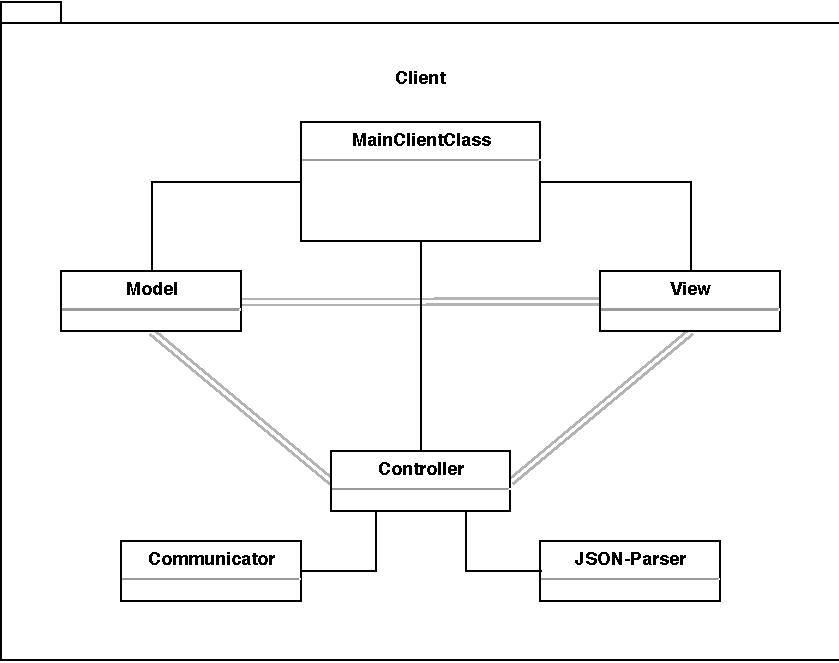
\includegraphics[scale=1]{images/Uebersicht.pdf}
    \end{figure}

\subsection{Beschreibung}
	Die Client Anwendung besteht aus den folgenden Klassen.
	Die Klassen Model, View und Controller 
		
\end{table}
    
	\section{Model}
	\subsection{Klassen-Diagramm}
	\begin{figure}[H]
        \centering
        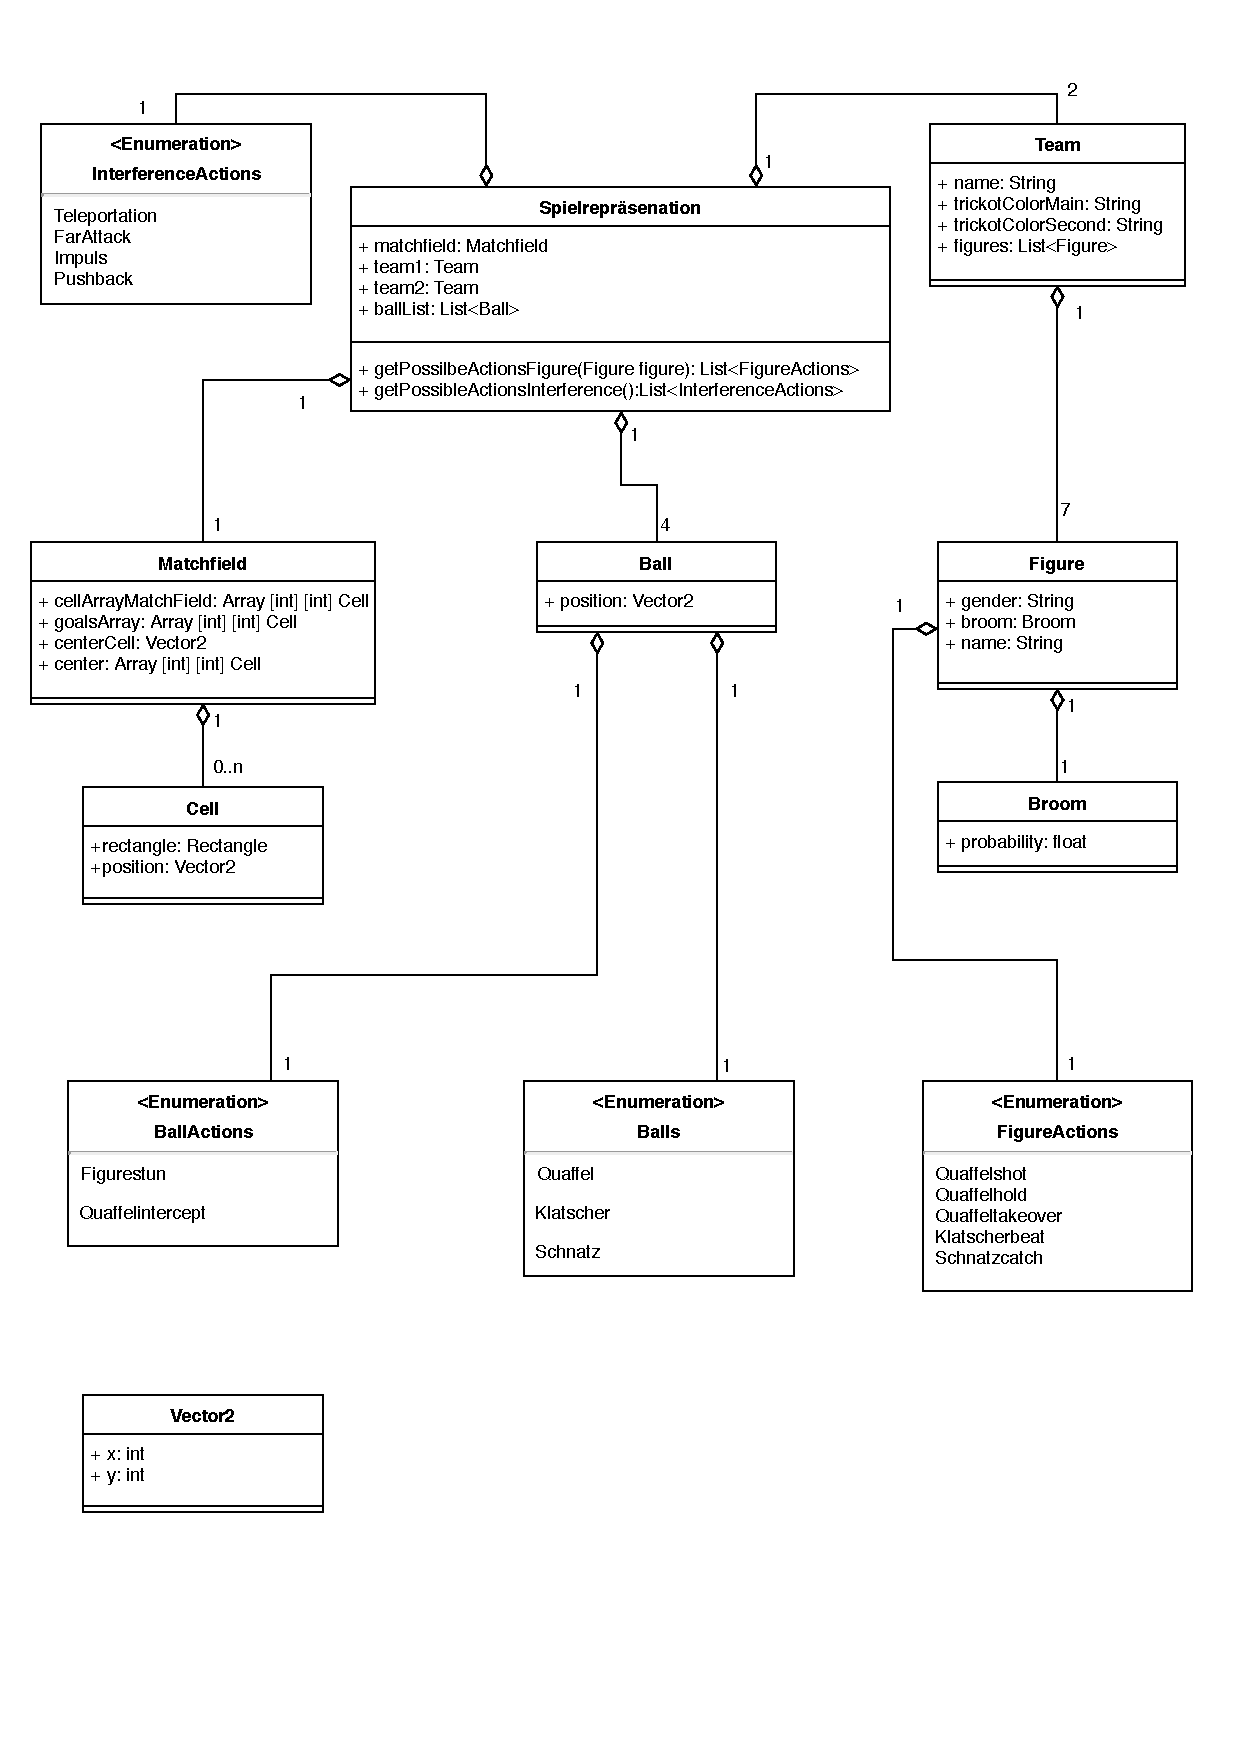
\includegraphics[scale=0.7]{images/model.pdf}
    \end{figure}

\subsection{Beschreibung}
Die Model ist für die Repräsentation für die Daten verantwortlich. Hier sind alle Daten hinterlegt, die für das Spiel relevant sind und angezeigt werden in der Benutzeroberfläche. Die Daten wertet der Controller aus und gibt diese dann der View weiter, welche diese dann auf der Benutzeroberfläche an.
	\subsubsection{Gamerepresentation (Klasse)}
	
		\begin{description}
                
			\item[Konstruktor]
			Der Konstruktor erstellt eine Instance des Objektes Gamerepresentation. In diesem Objekt sind alle Objekte die für das Spiel notwendig sind und auf dem Spielfeld agieren enthalten und jeweils eine Instanz erstellt.
                
        	\item[getPossibleActionsFigure (Methode)]
        	Diese public Methode hat den Zweck eine Liste zu erstellen, in der alle möglichen Aktionen aufgelistet werden, die eine übergebene Spielfigur machen kann. Dazu überprüft die Methode welchen Typ Figur die übergeben Spielfigur hat, und welche AKtionen sie dadurch durchführen darf und gibt diese als Liste wieder.
        	
        	\item[getPossibleActionsInterference (Methode)]
        	Diese public Methode gibt die in der Enumeration definierten Einmischungen als Liste zurück. Dazu liest sie die Enumeration ein und spiechert diese in einer Liste, welche dann zurückgegeben wird. 
        \end{description}
        	
        \subsubsection{Matchfield (Klasse)}
        \begin{description}
        	\item[Konstruktor]
        	In dem Konstruktor für das Matchfield, wird das eigentliche Spielfeld erstellt. Dazu erstellt diese Klasse ein Array von Zellen, welche das Spielfeld repräsentieren. Außerdem gibt es noch Bereiche, die besonders sind, aber auch Zellen auf dem Spielfeld sind. So sind die Torringe ebenfalls in einem Array hinterlegt, das Zentrum ist als Vektor hinterlegt und das Mittelfeld ist ebenfalls als Array hinterlegt.
        \end{description}
        
        \subsubsection{Team (Klasse)}
        \begin{description}
        	\item[Konstruktor]
        	Das Team ist ebenfalls Bestandteil der Klasse Gamerepresentation. In dem Team werden die 7 Spieler instantiiert, so wie der Name, die Trikotfarbe und die Ersatzfarbe für die Trikots.
        \end{description}
        
        \subsubsection{Ball (Klasse)}
        \begin{description}
        	\item[Konstruktor]
        	Durch die Klasse Ball wird ebenfalls in der Gamerepresentation ein Bestandteil des Spieles instantiiert. Die Bälle bestehen aus einer Enumeration, welche Bälle es gibt, so wie aus einer Position, die als Vektor repräsentiert wird. Außerdem besitzt die Klasse Ball noch eine Enumeration, welche Aktionen ein Ball machen kann.
        \end{description}

\subsection{Zuordnung der Funktionalen Anforderungen}

Die Funktionalen Anforderungen werden den Methoden folgendermaßen zugeteilt:


\begin{table}[h]
	\centering
	\begin{tabular}{|l|l|}
    	\hline
    	\textbf{Methode} & \textbf{Funktionelle Anforderungen} \\ \hline
    	getPossibleActionsFigure		&	FA21, FA24, FA26, FA28, FA30\\ \hline
    	getPossibleActionsInterference	&	FA32 - FA35\\ \hline

	\end{tabular}
\end{table}    
	 
	\section{View}
    \section{View}
\subsection{Klassendiagramm}
\begin{center}
	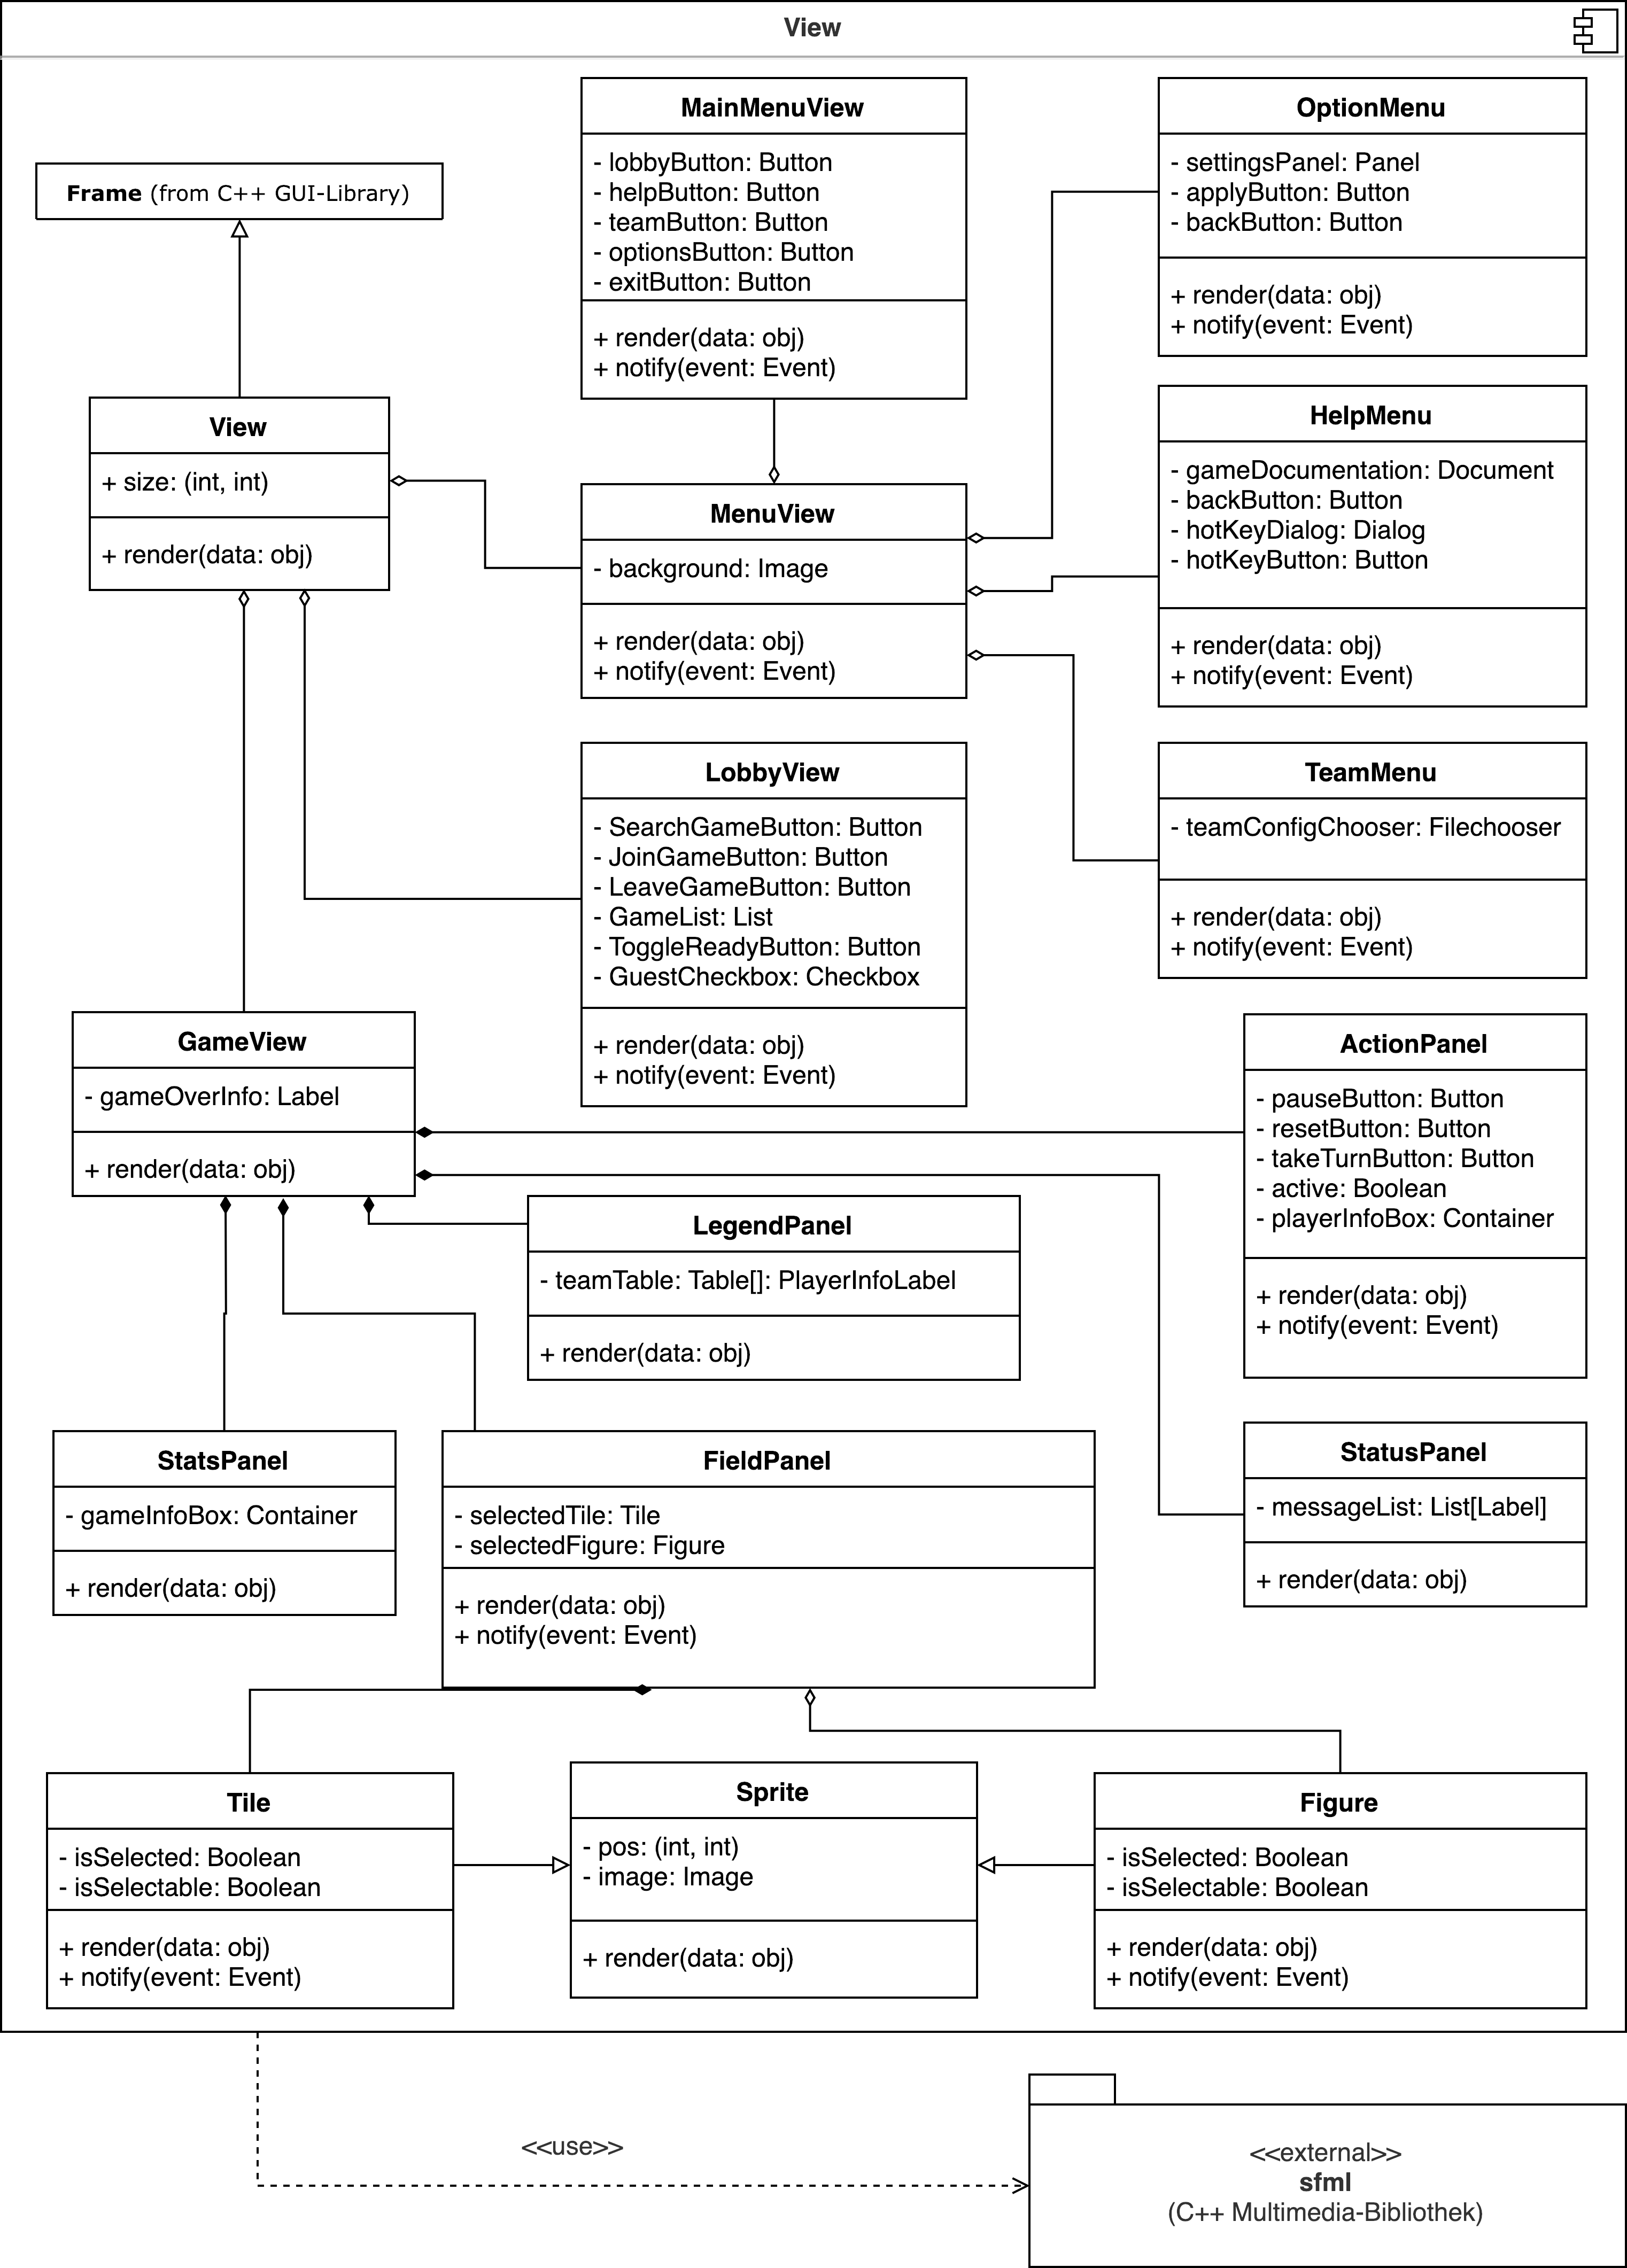
\includegraphics[width=14cm]{images/klassendiagramm_view_extended}
\end{center}

\subsection{Beschreibung}
	Die View dient lediglich als Schnittstelle zwischen Benutzer und Controller. Sie soll selbst keine Logik enthalten und basierend auf den Daten des Models den aktuellen Spielzustand anzeigen. 
	Im Folgenden werden die eingetragenen Methoden erklärt. Da in der gesamten Komponente der View auf eine externe Bibliothek zurückgegriffen werden wird, ist dies auf dem Diagramm entsprechend angedeutet.
\begin{description}
	\item[render (Methode)]
		Die render-Methode von Klassen in der View rendert bei jedem Aufruf die enthaltenen Objekte auf dem Anwendungsfenster.
	\item[notify (Methode)]
		Die notify-Methode von Klassen in der View leitet die entsprechenden Events der Elemente in der GUI an den Controller weiter.
	
	\item[sfml (externe Bibliothek)]
		Bei sfml handelt es sich um eine portable API für C++. Insgesamt stellt es eine komplette Multimedia-Bib liothek dar. Hier wird es als Fenster-Manager und GUI-Bibliothek sowie zur Darstellung von 2D-Grafik-Objekten und ggf. zum Abspielen von Musik verwendet.
		Da eine endgültige Festlegung auf diese Bibliothek noch nicht stattgefunden hat, ist ihre Verwendung auf dem Klassendiagramm nur angedeutet und noch nicht fest eingearbeitet. Die Bezeichnungen der entsprechenden Klassen im Diagramm sind daher möglichst allgemein gehalten.
\end{description}


\subsection{Zuordnung der funktionalen Anforderungen}
Die Funktionalen Anforderungen werden den Methoden folgendermaßen zugeteilt:
\begin{center}
	\begin{tabular}{|l|l|}
		\hline
		\textbf{Funktionale Anforderungen} & \textbf{Methoden}\\\hline
		FA60 & MainMenuView::render\\
		FA61& LobbyView::render\\\hline
		FA62 & GameView::render\\\hline
		FA63 & TeamMenu::render, TeamMenu::notify\\\hline
		FA64 & GameView::render\\\hline
		FA65 & HelpMenu::render\\\hline
		FA66 & GameView::render\\\hline
		
	\end{tabular}
\end{center}

    
    \section{Controller}
	\subsection{Klassendiagramm}
\begin{center}
	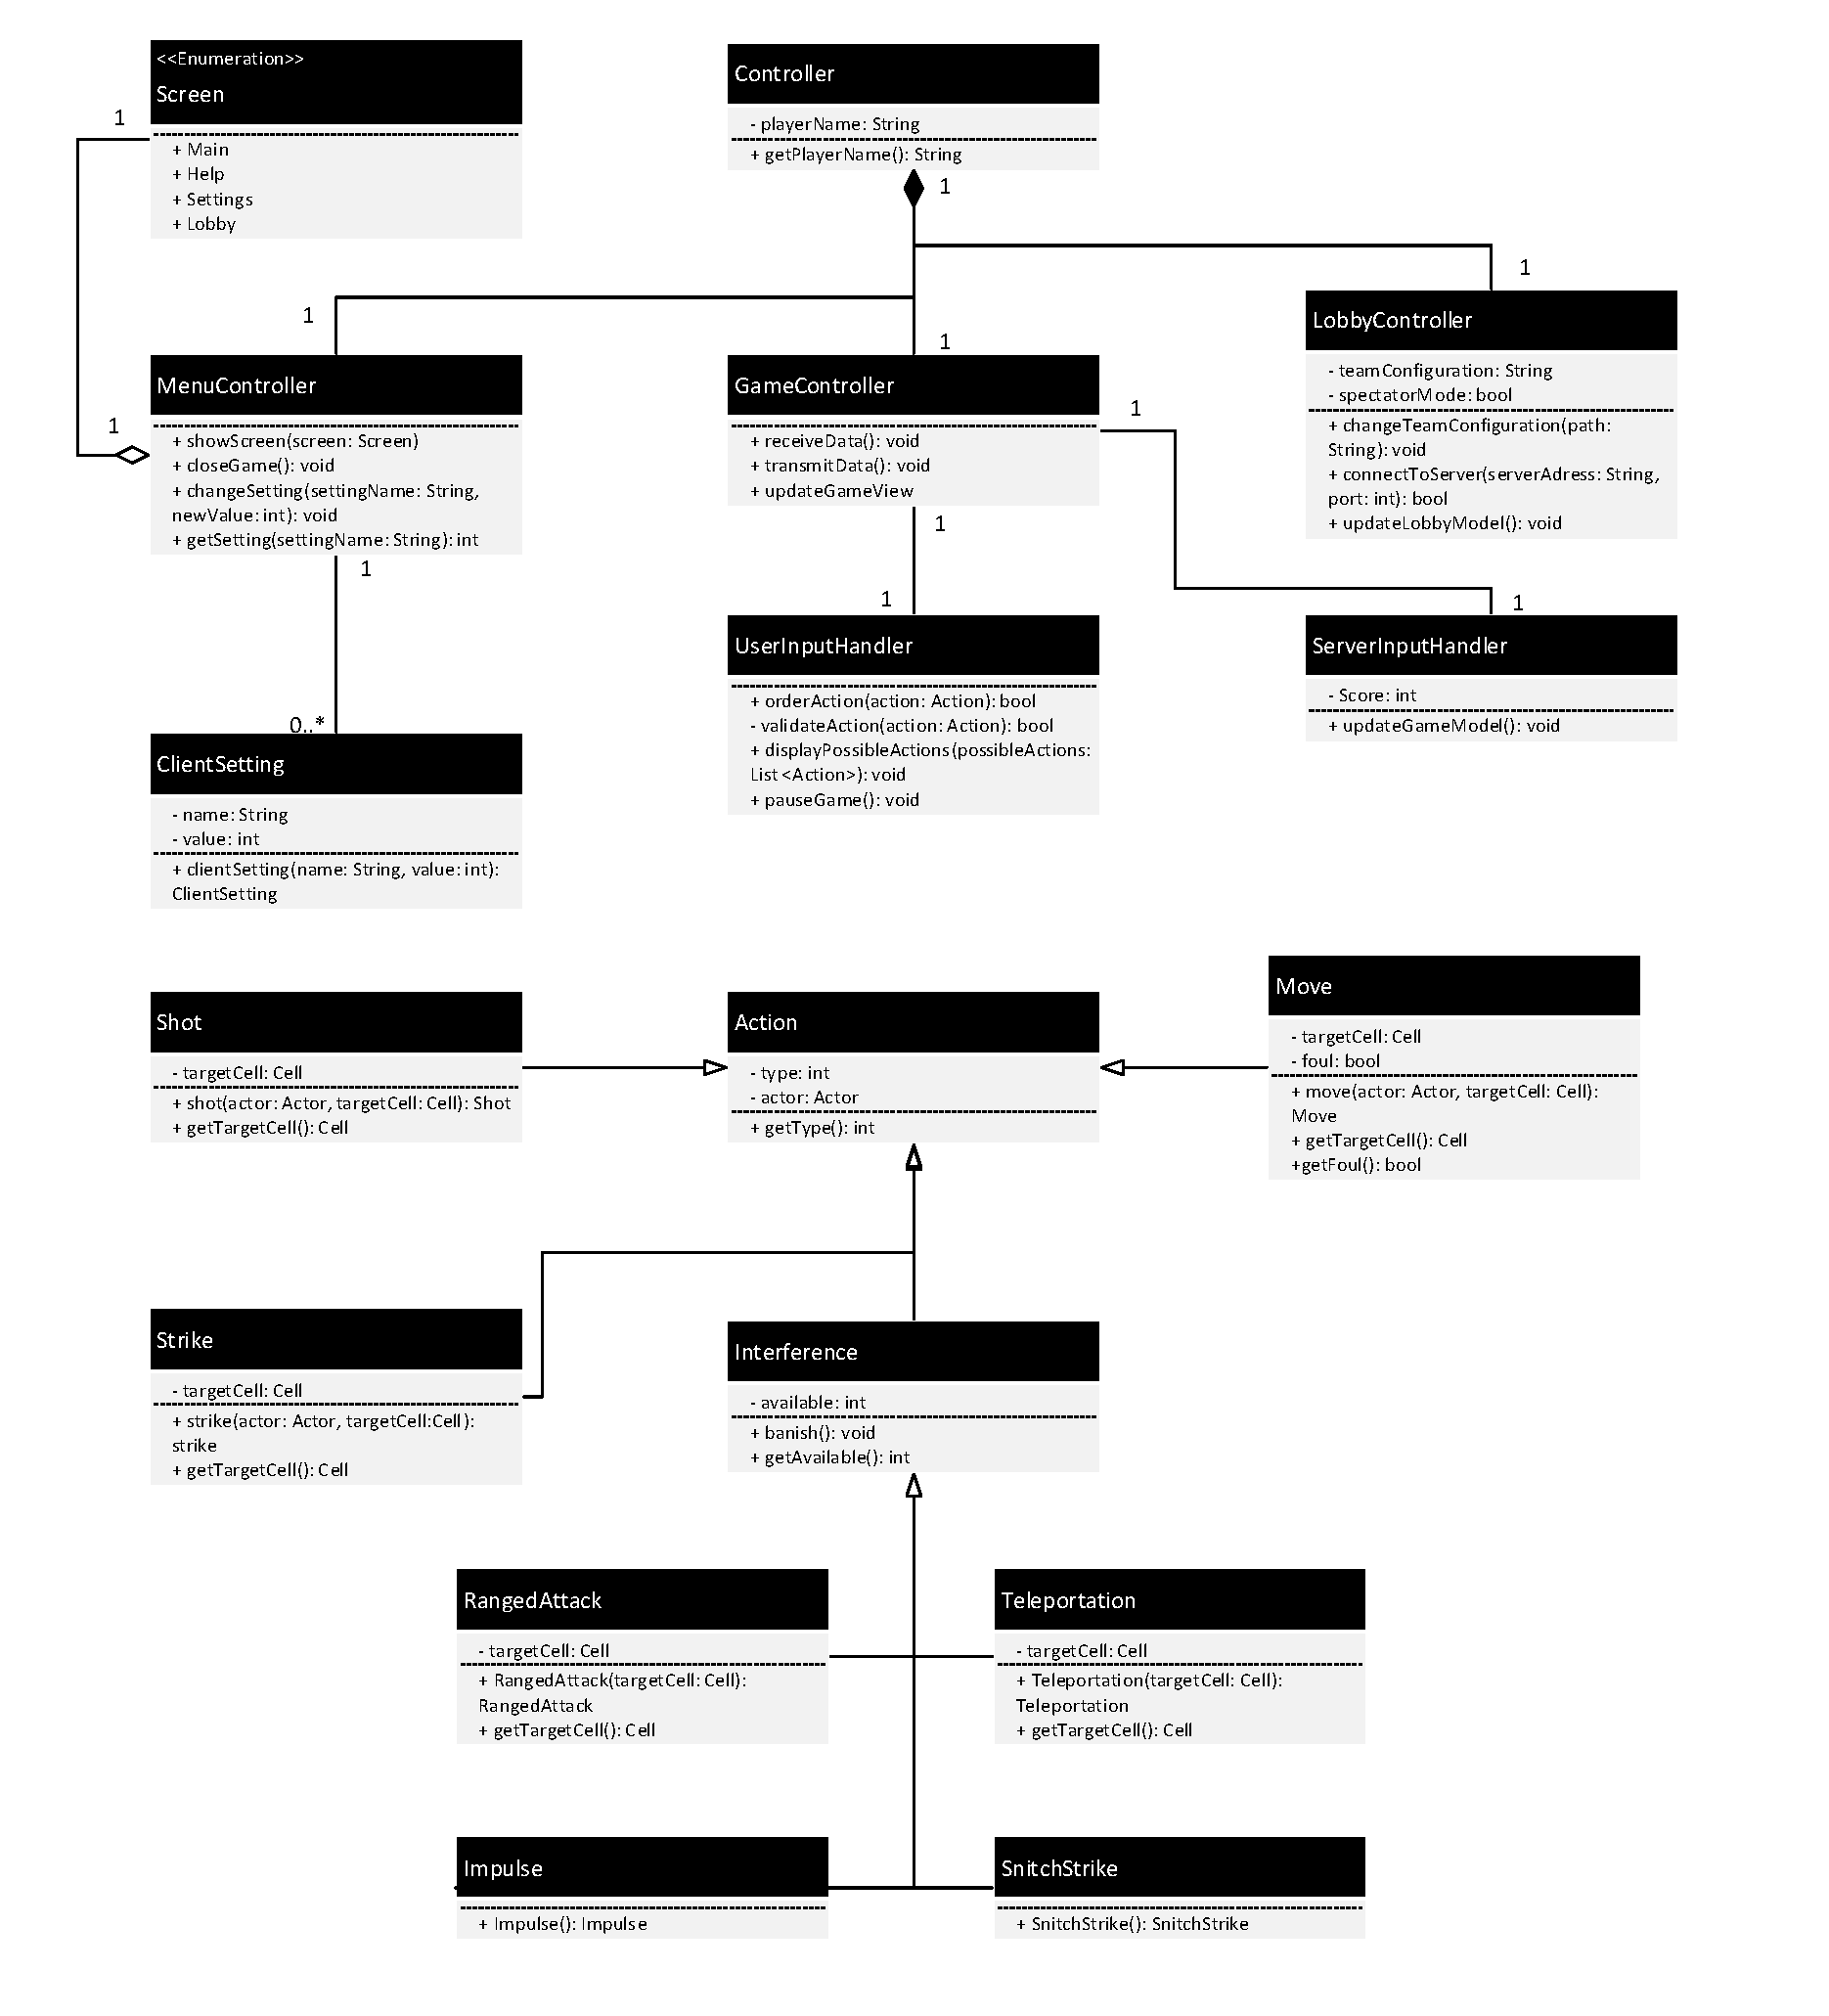
\includegraphics[width=16.8cm]{images/Klassendiagram_Controller}
\end{center}
\subsection{Beschreibung}
	Im Folgenden werden die eingetragenen Methoden erklärt.
\begin{center}
	\begin{tabular}{|p{4.0cm}|p{2.2cm}|p{2.2cm}|p{4.7cm}|}
		\hline
		\textbf{Name} & \textbf{Vorbedin-gungen} & \textbf{Nachbedin-gungen} & \textbf{Erklärung}\\\hline
		\multicolumn{4}{|l|}{\textbf{MenuController}} \\\hline
		closeGame & - & Positive Antwort in einem Popup-Fenster & Beendet die Anwendung\\\hline
		changeSetting & ClientSetting mit dem angegebenen settingName existiert & Der Wert von newValue wird akzeptiert & Ändert das Attribut value des ClientSetting mit dem Attribut name, der dem Parameter settingName entspricht, auf den Wert des Parameters newValue.\\\hline
		getSetting& ClientSetting mit dem angegebenen settingName existiert & - & Liefert den derzeitigen Wert des Attributs value des ClientSetting, dessen Attribut name mit dem Parameter settingName übereinstimmt.\\\hline
		\multicolumn{4}{|l|}{\textbf{GameController}} \\\hline
		receiveData & - & - & Empfängt Daten vom JSON-Parser und übergibt sie dem ServerInputHandler\\\hline
		transmitData & - & - & Empfängt Daten vom UserInputHandler und sendet sie über den JSON-Parser und den Kommunikator zum Server\\\hline
		\multicolumn{4}{|l|}{\textbf{LobbyController}} \\\hline
		changeTeamCon-figuration & - & Parameter path ist ein gültiger Pfad zu einer Team-Konfigurations-Datei & Ändert den Wert von teamConfiguration, in dem der Pfad zu der zu verwendenden Team-Konfigurations-Datei gespeichert ist.\\\hline
		
	\end{tabular}
	
	\begin{tabular}{|p{4.0cm}|p{2.2cm}|p{2.2cm}|p{4cm}|}	
		\hline
		connectToServer & Parameter serverAdress und port sind ungleich Null & - & Veranlasst über den JSON-Parser den Kommunikator dazu, eine Verbindung mit dem in den Parametern spezifiziertem Server aufzubauen. Gibt true zurück, wenn der Verbindungsaufbau erfolgreich war, ansonsten false.\\\hline
		\multicolumn{4}{|l|}{\textbf{UserInputHandler}} \\\hline
		validateAction & - & - & Fordert vom Partie-Model Daten an und entscheidet danach, ob die geforderte Action durchgeführt werden kann. Gibt true zurück wenn die als Parameter übergebene Action gültig ist, ansonsten false.\\\hline
		orderAction & validateAction gibt für die als Parameter übergebene Action true zurück. & - & Übergibt die auszuführende Aktion an den GameController. Ruft die Methode validateAction auf und gibt deren Rückgabewert zurück.\\\hline
		displayPossibleActions & - & - & Fordert vom Partie-Model Daten an und berechnet alle möglichen Aktionen und gibt sie an die Partie-View weiter, um sie dem Spieler anzuzeigen.\\\hline
		\multicolumn{4}{|l|}{\textbf{Interference}} \\\hline
		banish & - & - & Verringert das Attribut available um eins.\\\hline
		
	\end{tabular}
\end{center}
\subsection{Zuordnung der Funktionalen Anforderungen}
Die Funktionalen Anforderungen werden den Methoden folgendermaßen zugeteilt:
\begin{center}
	\begin{tabular}{|l|l|}
		\hline
		\textbf{Funktionale Anforderungen} & \textbf{Methoden}\\\hline
		FA7 & Shot::shot\\
		& Shot::getTargetCell\\\hline
		FA21 & Shot::shot\\\hline
		FA26 & Move::move\\\hline
		FA27 & Shot::shot\\\hline
		FA28 & Strike::strike\\\hline
		FA30 & Move::move\\\hline
		FA31 & RangedAttack::rangedAttack\\
		& Teleportation::teleportation\\
		& Impulse::impulse\\
		& SnitchStrike::snitchStrike\\
		& Inteference::banish\\\hline
		FA32 & Teleportation::teleportation\\\hline
		FA33 & RangedAttack::rangedAttack\\\hline
		FA34 & Impulse::impulse\\\hline
		FA35 & SnitchStrike::snitchStrike\\\hline
		FA36 & Inteference::banish\\
		& Actor::setBanished\\\hline
		FA37 & Actor::setBanished\\
		& Move::move\\\hline
		FA38 - FA42 & Move::move\\\hline
		FA48 & Actor::setBanished\\\hline
		FA54 & LobbyController::changeTeamConfiguration\\
		& LobbyController::updateLobbyModel\\\hline
		FA55 & GameController::receiveData\\
		& GameController::transmitData\\
		& LobbyController::connectToServer\\\hline
		FA56 & GameController::receiveData\\
		& GameController::transmitData\\\hline
		FA60-FA61 & MenuController::showScreen\\\hline
	\end{tabular}

	\begin{tabular}{|p{5.5cm}|l|}
		\hline
		FA67 & UserInputHandler::orderActions\\
		& UserInputHandler::validateActions\\
		& MenuController::showScreen\\
		& MenuController::changeSetting\\
		& LobbyController::changeTeamConfiguration\\
		& LobbyController::connectToServer\\\hline
		FA69 & UserInputHandler::pauseGame\\\hline
		
	\end{tabular}
\end{center}
    
    
    \section{Kommunikator}
    \subsection{Klassen-Diagramm}

    \begin{figure}[H]
        \centering
        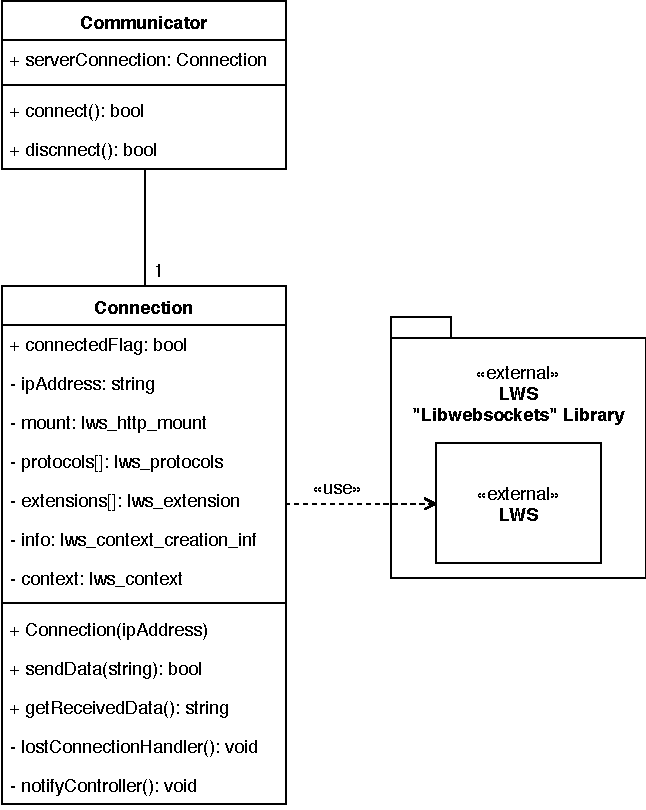
\includegraphics[scale=1]{images/Kommunikator.pdf}
    \end{figure}
    
    \newpage

\subsection{Beschreibung}
	\subsubsection{Connector (Klasse)}
	
		Im Allgemeinen dient die Connector Klasse dazu, die Kommunikation zwischen der Client Anwendung und der Server Anwendung über das Netzwerk zu verwalten. 
	
		\begin{description}
                
        	\item[connect (Methode)]
        	Die connect Methode dient dazu, eine neue Verbindung mit einem Server aufzubauen. Die IP-Adresse des Servers wird dabei als Parameter übergeben. Ist die Aktion erfolgreich, so wird true zurück gegeben, anderenfalls false.
			
			\item[disconnect (Methode)]
        	Die disconnect Methode dient dazu, eine bestehende Verbindung mit einem Server zu trennen. Ist die Aktion erfolgreich, so wird true zurück gegeben, anderenfalls false.
        	
    	\end{description}
	
	\subsubsection{Connection (Klasse)}    	
	
		\begin{description}
                
        	\item[sendData (Methode)]
        	Die öffentliche sendData Methode dient dazu, einen im JSON-Format formatierten String an den Server zu übertragen. Ist die Aktion erfolgreich, so wird true zurück gegeben, anderenfalls false. Zur Umsetzung dieser Methode werden Funktionen und Strukturen der Drittanbieter-Bibliothek LWS benötigt.
        	
        	\item[getReceivedData (Methode)]
			Mit Hilfe der öffentlichen Methode getReceivedData kann der letzte vom Server gesendete JSON Datensatz ausgelesen werden. Zur Umsetzung dieser Methode werden ebenfalls Funktionen und Strukturen der Drittanbieter-Bibliothek LWS benötigt.    	
        	
        	\item[lostConnectionHandler (Methode)]
			Die private Methode lostConnectionHandler kümmert sich im Falle eines außerplanmäßigen Verbindungsverlust darum, dass alle notwendigen Schritte eingeleitet werden, indem der Controller über den Verbindungsabbruch informiert wird. Auch hier werden zur Umsetzung Funktionen und Strukturen der Drittanbieter- Bibliothek LWS benötigt.          	
        	
        	\item[notifyController (Methode)]
        	Die private notifyController Methode ist dafür zuständig den Controller über das Eingehen von neuen Nachrichten des Servers zu informieren.
        	
    	\end{description}
    	
    \subsubsection{LWS (Externe Bibliothek)}
		Bei dieser Klasse Handelt es sich um eine externe Bibliothek, die verschiedenste Methoden und Strukturen zur Verfügung stellt um in einem C/C++ Projekt einfache Server Client Verbindungen mittels Web-Sockets zu implementieren. Genauere Informationen zu dieser Bibliothek sind unter folgendem Link zu finden: \\ \url{https://libwebsockets.org/}

\subsection{Zuordnung der Funktionalen Anforderungen}

Die Funktionalen Anforderungen werden den Methoden folgendermaßen zugeteilt:

\begin{table}[h]
	\centering
	\begin{tabular}{|l|l|}
    	\hline
    	\textbf{Funktionale Anforderungen} & \textbf{Methoden} \\ \hline
		FA55 & Connector::connect \\ \hline
    	FA55 & Connector::disconnect \\ \hline    	
    	FA55 & Connection::sendData \\ \hline
    	FA55 & Connection::getReceivedData \\ \hline
    	FA55 & Connection::lostConnectionHandler \\ \hline
    	FA55 & Connection::notifyController \\ \hline

	\end{tabular}
\end{table}  
    
    \section{JSON-Parser}
    \subsection{Klassen-Diagramm}
	\begin{figure}[H]
        \centering
        
\includegraphics[scale=1]{images/JSON-Parser.pdf}
    \end{figure}

\subsection{Beschreibung}

	\subsubsection{JSON-Parser (Klasse)}
	
		Der JSON-Parser übernimmt das Serialisieren und Deserialisieren von Objekten in einen String im JSON-Format. Diese Funktionalität wird benötigt, da alle Daten, die über das Netzwerk versendet werden oder aus einer Datei eingelesen werden diesem Format entsprechen müssen.
	
		\begin{description}
                
        	\item[deserialize (Methode)]
        	Die private deserialize Methode dient dazu, einen dem JSON-Format konformen String in ein JSON-Object umzuwandeln. Dabei wird bei der Umsetzung dieser Funktionalität auf Methoden und Strukturen aus einer Softwarebibliothek eines Drittanbieters zurückgegriffen. 
        	
        	\item[serialize (Methode)]
        	Die private serialize Methode dient dazu, aus einem JSON-Object ein dem JSON-Format genügenden String zu erzeugen. Wie auch schon bei der deserialize Methode wird dabei auf Methoden und Strukturen aus einer Softwarebibliothek eines Drittanbieters zurückgegriffen. 
        	
        	\item[readTeamConfig (Methode)]
        	Mit Hilfe der readTeamConfig Methode kann die Team-Konf-iguration aus der Team-Konfigurationsdatei eingelesen werden und in ein internes TeamObject umgewandelt werden. Diese wird dann im Model hinterlegt. Im Hintergrund greift diese Methode auf die deserialize Methode zurück.
        	
        	\item[convertJsonToTeamObject (Methode)]
        	Die convertJsonToTeamObject Methode dient dazu, die vom Server empfangenen Daten über das gegnerische Team in ein internes TeamObject umzuwandeln. Diese wird dann im Model hinterlegt. Im Hintergrund greift diese Methode auf die deserialize Methode zurück. 
        	\item[convertTeamObjectToJson (Methode)]
        	Die convertGameDataToJson Methode bildet das Gegenstück zur convertJsonToTeamObject Methode. Es kann also ein internes GameTeam in einen JSON konformen String konvertiert werden, welcher dann an den Server versendet werden kann. Im Hintergrund greift diese Methode auf die serialize Methode zurück.
        	
        	\item[convertJsonToGameData (Methode)]
        	Die convertJsonToGameData Methode dient dazu, die vom Server empfangenen Daten über das aktuelle Spielgeschehen aus dem JSON-Format in ein Internes GameObject zu konvertieren. Diese wird dann im Model hinterlegt. Im Hintergrund greift diese Methode auf die deserialize Methode zurück. 

			\item[convertGameDataToJson (Methode)]
        	Die convertGameDataToJson Methode bildet das Gegenstück zur convertJsonToGameData Methode. Es kann also ein internes GameObject in einen JSON konformen String konvertiert werden, welcher dann an den Server versendet werden kann. Im Hintergrund greift diese Methode auf die serialize Methode zurück. 
        	
    	\end{description}
    	
    \subsubsection{nlohmann::json (Externe Bibliothek)}
		Bei dieser Klasse Handelt es sich um eine externe Bibliothek, die verschiedenste Methoden und Strukturen zur Verfügung stellt um in einem C++ Projekt mit Objekten mit JSON-Struktur einfach zu arbeiten. Vermutlich wird die von \textit{Niels Lohmann} entwickelte freie JSON Bibliothek namens \textit{JSON for Modern C++} verwendet werden. Genauere Informationen zu dieser Bibliothek sind unter folgendem Link zu finden: \\ \url{https://github.com/nlohmann/json}

\subsection{Zuordnung der Funktionalen Anforderungen}

Die Funktionalen Anforderungen werden den Methoden folgendermaßen zugeteilt:


\begin{table}[h]
	\centering
	\begin{tabular}{|l|l|}
    	\hline
    	\textbf{Funktionale Anforderungen} & \textbf{Methoden} \\ \hline
    	FA54 & readTeamConfig \\ \hline
    	FA54 & convertJsonToTeamObject \\ \hline
    	FA54 & convertTeamObjectToJson \\ \hline
    	FA53 & convertGameDataToJson \\ \hline
    	FA53 & convertJsonToGameData \\ \hline

	\end{tabular}
\end{table}

\end{document}

